\documentclass[12pt,a4paper]{amsart}
%\usepackage[norsk]{babel}
\usepackage[english]{babel}
\usepackage[utf8]{inputenc}
%\usepackage[fleqn]{amsmath}
\usepackage{amsmath}
\usepackage[T1]{fontenc}
\usepackage{mathtools}
\usepackage{graphicx}
\usepackage{subcaption}
\usepackage{verbatim}
\usepackage{listings}
\usepackage{scalerel}
\usepackage{fixltx2e}
\usepackage{amssymb}
\usepackage{siunitx}
\usepackage{xfrac}
\usepackage{enumitem}
\usepackage{hyperref}
\usepackage{float}
\usepackage{bbold}
\usepackage{physics}
\usepackage[ampersand]{easylist}
\usepackage{subcaption}
\usepackage{wrapfig}
\usepackage{algorithmicx}
\usepackage{csquotes}
\usepackage{xcolor}

%%For visualizations of table
\usepackage{multirow}
\usepackage{arydshln}
\usepackage{booktabs}

\usepackage[english]{babel}\addto\captionsenglish  
{\renewcommand{\bibname}{References}}  
\usepackage[backend=bibtex,style=phys]{biblatex}  %backend=biber is 'better'  
%\usepackage[backend=biber]{biblatex}
%\usepackage{apacite}
\addbibresource{graviton_analysis.bib}

\usepackage[margin=1.5in]{geometry}
\newcommand{\scalel}{\scaleleft{<}}
\newcommand{\scaler}{\scaleright{>}}

%% physics packages
\usepackage{physics}
\usepackage[compat=1.1.0]{tikz-feynman}
\usepackage{feynmf}

% adjust the spacing around figure if pdf-file with white space:
\usepackage[font=small,skip=0pt]{caption}
%\usepackage[margin=1.4in]{geometry}
%\captionsetup[figure]{skip=-100pt}

% define colors for text
\definecolor{mygreen}{RGB}{28,172,0} % color values Red, Green, Blue
\definecolor{mylilas}{RGB}{170,55,241}
\definecolor{forestgreen}{rgb}{0.13, 0.55, 0.13}

% definitions of commands
%\renewcommand{\thesection}{\arabic{section}}

%\makeatletter
%\patchcmd{\@settitle}{\uppercasenonmath\@title}{}{}{}
% layout for sections, subsections and subsubsections
\usepackage{titlesec} % Allows customization of titles
\renewcommand\thesection{\Roman{section}} % Roman numerals for the sections
\renewcommand{\thesubsection}{\Alph{subsection}} % Alphabetic letters for the subsections
\renewcommand{\thesubsubsection}{\arabic{subsubsection}} % Arabic numerals for the subsubsections
\titleformat{\section}[block]{\normalfont\scshape\centering\bfseries}{\thesection.}{1em}{} % Change the look of the section titles
\titleformat{\subsection}{\normalsize\large\filcenter\bfseries}{\thesubsection.}{1em}{}
\titleformat{\subsubsection}[runin]{\medium\bfseries}{\thesubsubsection.}{1em}{}% Change the look of the section titles

\title[OpenData dilepton analysis - graviton]{Project 3: \\ Search for graviton resonances at $\sqrt{s} = 13\si{TeV}$ using ATLAS Open Data\\
\small{\mdseries FYS5555 - Spring 2020}}
\date{\today}
\author[Christensen]{Elisabeth Christensen}

\begin{document}
\maketitle
\begin{abstract}
...
\end{abstract}

\section{Introduction}
In the search for a unified \textit{theory of everything}, one must overcome the question of gravitation and the relation between the two grand theories derived within physics thus far. One of which, dedicated to describe the universe on a macroscopic level and the gravitational forces within, known as general theory of relativity, and the other, dedicated to describe the fundamental forces at a quantum level, known as the Standard Model.

The general theory of relativity, as proposed by Albert Einstein~\cite{Einstein:1915}, emerged in 1915 in a (highly succesful) attempt to describe the gravitational interactions of matter. The Standard Model~\cite{Thomson:2019} on the other hand, emerged as a result of the tedious calculations of quantum field theory, and has for the past 50 years proven a valid model describing the interactions of elementary particles and the forces acting between them. So far, the Standard Model has achieved in describing, with great accuracy, three of the four fundamental forces of nature. This concludes the electromagnetic force, the weak force, and the strong force which came into place during the 1970s upon the experimental evidence of quarks. The latest contribution to the Standard Model being the Higgs boson, upon its discovery in 2012. However, it has so far not been able to account for the fourth fundamental force, i.e. gravity. This is due to the infinities arising from the singularities in Feynman diagrams~\cite{PhilosophyMeetsPhysics:2001}, which, unlike in QED and QCD, cannot be renormalized away.

However, there are multiple theories devoted to solve such a problem. One of which is based on string theory, and will be the theory which allows us to search for not only graviton resonances in a proton-proton collision, but also higher dimensions apart from time and the three spatial dimensions familiar to us today. We will in this report study the production and decay of gravitons to two leptons ($q\bar{q}\rightarrow G^* \rightarrow l^+l^-$), at a resonance range between 750-4000GeV, by the use of Monte Carlo simulations of the graviton based on the Randall-Sundrum model and observed data obtained from the \textit{ATLAS Open Data} source. The ATLAS Open Data source provides both observed and simulated data events, using Monte Carlo, of pp collisions at an integrated luminosity of $10\si{fb}^{-1}$.

\section{Theory}
\subsection{Graviton resonances}
(Kaluza-Klein towers, RS-model emerging from Kaluza-Klein theory)
\subsection{Collider physics}
In order to test a theory within particle physics we must know what to look for and how to look for it. A tool that helps us tremendously along the way is a particle detector. A particle detector allows for the detection, identification and track of the decay products emerging from a collision. An example of this is the ATLAS detector, which will provide the dataset for our analysis. \\

\textbf{ATLAS Detector.} The ATLAS detector consists mainly of an inner tracking detector, hadronic and electromagnetic calorimeters measuring the energy lost by the charged particles as they move through matter, and a muon spectrometer. The layout within ATLAS can be seen in the 2D-scheme from figure~\ref{fig:ATLAS_layout_2D}. Here, the pixel/SCT detector and the transitioan radiation tracker consitutes the inner parts of ATLAS, and are the first components to track the decay products of the p-p collisions. They measure, among other things, the momentum and charge of the particles, with the solenoid magnet assisting in the momentum measurements. As the particles move further out from the inner detector they reach the electromagnetic (EM) calorimeter. The EM calorimeter measures the energy deposited by any charged particle, except muons due to the density of the liquid argon used within the detector. Hadrons, such as the proton and neutron, carry enough energy to make it past the EM calorimeter and move on to the hadronic calorimeter. The hadronic calorimeter consists of iron plates and scintillating tiles~\cite{hadronic_calorimetry}, where the scintillation light, produced by the energy deposited from hadrons, is read out by photomultiplier tubes. Lastly, any particles that makes it through the calorimeters, i.e. muons and neutrinos, reach the outer layers of the detector, that is the muon spectrometer. The muon spectrometer consists of a large array of muon chambers each dedicated to identify and measure the momentum of the passing muons. \\

\begin{figure}
\centering
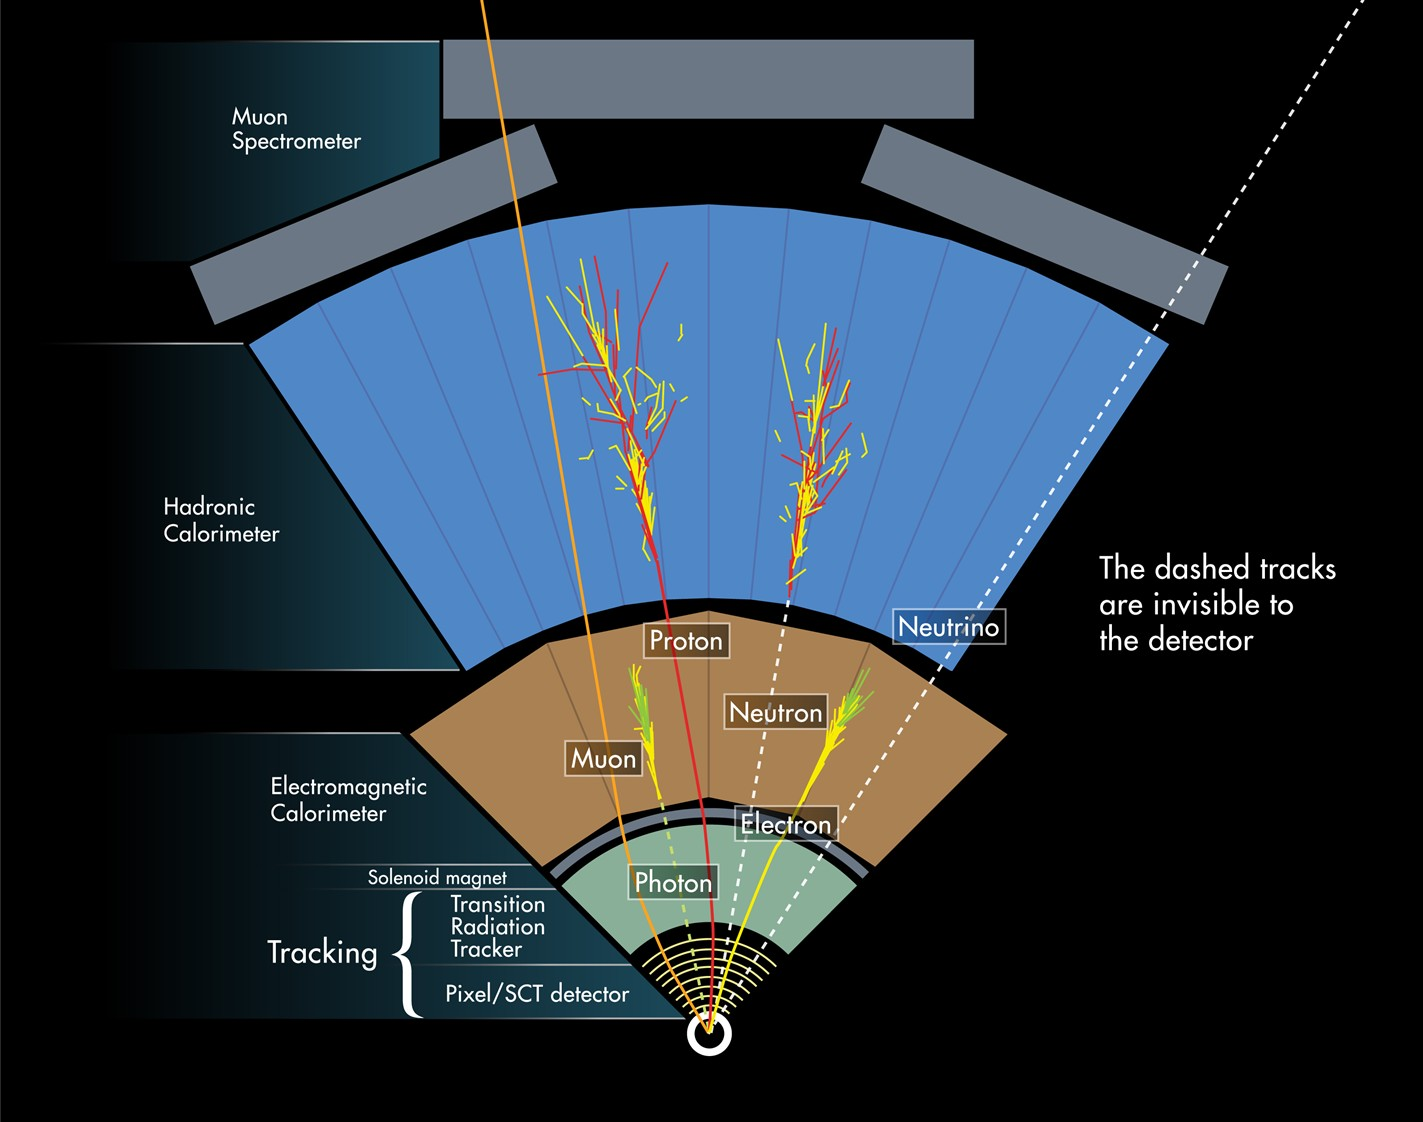
\includegraphics[width=.8\textwidth]{figures/ATLAS_layout_2D.jpg}
\caption{2D layout of the ATLAS detector.~\cite{ATLAS_2D}}
\label{fig:ATLAS_layout_2D}
\end{figure}

\textbf{Kinematic properties.}  A few definitions of the parameters used in our dataset are in order. To start, we operate with polar angle $\theta$ and azimuthal angle $\phi$ to describe the trajectories of the particles within the detector. In a p-p collision, the center-of-mass frame is between the initial hadrons, i.e. the protons, and \textit{not} between the colliding partons themselves. Because of this, we can introduce a variable known as the rapidity, $y$, where the differences of rapidity are invariant under boosts along the beam direction~\cite{Thomson:2019}. (This insures that any longitudinal boost in a parton-parton system will not have an effect on the distribution of rapidity differences.) The rapidity is defined as
\begin{align}
y = \frac{1}{2}\ln\left(\frac{E+p_z}{E-p_z}\right) \label{eq:rapidity}
\end{align}
where the measured quantities $E$ and $p_z$ represents respectively the energy and the z-component of momentum of a jet. For high-energy jets, where the jet masses can be neglected, we can use what is known as the pseudorapidity, $\eta$, where $p_z\approx E\cos\theta$, such that
\begin{align}
\eta = -\ln (\tan\frac{\theta}{2}). \label{eq:pseudorapidity}
\end{align}

There are several factors involved in order to establish the energy measurements in a detector. Any missing energy may indicate either a mis-measurement, poor detector coverage or particles escaping the detector before a proper identification is made, such as neutrinos. The missing energy is often based on the missing transverse energy, $E_T^{miss}$ as any longitudinal energy that goes undetected are generally poorly measured~\cite{Green:2004}.

In order to accurately describe any physics at the interaction point of our collision, we must restrict ourselves to partons directly interacting with one another. This is done by measuring the transverse momentum, $p_T$, as any partons not involved in a collision will continue along the beam line, with the initial longitudinal momentum as before the interaction point. Thus, high transverse momentum may be an indication of high mass phenomenas, i.e. potential new physics.


\textbf{Precision of detector.} The resolution of the detector determines the sensitivity for new discoveries. The tracking and energy resolution are defined as 
\begin{align}
\frac{dP}{P} = cP\oplus d, \hspace{.5cm}\frac{dE}{E}&= a/\sqrt{E}\oplus b \label{eq:resolution}
\end{align}
where $c$ corresponds to the deflection angle of a particle in the magnetic field, while the factor $d$ describes multiple scattering. $a$ describes the stochastic fluctuations in the energy, while $b$ describes the non-uniformity of the medium.

\subsection{Statistical physics}
In order to study the correlation between our dataset and the theory we can make use of Bayesian statistics. Here, we can treat a parameter $\theta$ as random. This thus allows us to compute a probability, after observing the data $x$, corresponding to the credibility of observing $\theta$ within a certain interval. As an example, if our probability to observe $\theta$ within an interval is $95\%$ after observing the data, then we refer to this as a $95\%$ credible interval. A credible interval of size $1-\alpha$ is referred to as an interval between $a$ and $b$, where
\begin{align}
P(a\leq \theta \leq b|x) = 1-\alpha	\label{eq:credible_interval_one_sided}
\end{align}
with $\alpha$ corresponding to the one-sided tail of a distribution. In the case of a two-sided tail, our credible interval is defined by
\begin{align}
P(\theta<a|x) = \alpha/2, \hspace{.5cm} P(\theta > b|x) = \alpha/2.	\label{eq:credible_interval_two_sided}
\end{align}
Bayesian statistics allows us to produce an upper limit on the amount of signal events, $s_{up}$, required in order for the true parameter to lie within our credible interval. In doing so, we can test the hypothesis $H_1$ (signal+background), vs the null hypothesis $H_0$ (background).

Bayes theorem states that
\begin{align}
p(\theta|x) = \frac{P(x|\theta)p(\theta)}{\int P(x|\theta)p(\theta)d\theta} \label{eq:Bayes}
\end{align}
Here, $p(\theta|x)$ corresponds to the \textit{posterior density function}, $P(x|\theta)$ is the likelihood function based on a given dataset and $p(\theta)$ corresponds to the \textit{prior probability function}. The integral in the denominator is included for normalization. The prior probability function depends on our prior knowledge of the system, which, in our case, will correspond to a Poisson distribution. The posterior density function thus tells us how probable our hypothesis $\theta$ given the data and our prior knowledge of the system. The more informative our prior is, the greater its influence on the posterior. The greater our sample size is, the greater the effect of the likelihood function on the posterior.

For our analysis, we will make use of the Bayesian single-bin limit setting. The likelihood function can then be expressed as
\begin{align}
P(x|\theta) = L(s) = P(n_{obs}|s) = \frac{\lambda^{n_{obs}} e^{-\lambda}}{n_{obs}!}, \hspace{.5cm}\lambda=s+b	\label{eq:likelihood}
\end{align}
where $s$ is the expected signal, $b$ is the expected background and $n_{obs}$ is the actual number of observed events. In the case of background uncertainty we can use the \textit{joint posterior}, where we include a prior, $p(b)$, on the uncertainty. The joint posterior is expressed as
\begin{align}
p(s, b|n_{obs}) = \frac{P(n_{obs}|s, b)p(s)p(b)}{P(n_{obs})}	\label{eq:joint_posterior}
\end{align}
while $\lambda$ can be expressed as 
\begin{align}
\lambda = L_{int}(\varepsilon_{sig}\sigma + \sigma^{eff}_{bkg})
\end{align}
where $L_{int}$ is the integrated luminosity, $\sigma$ is the signal cross-section with $\varepsilon_{sig}$ being the signal efficiency. The likelihood $L(\sigma, L_{int}, \varepsilon_{sig}, \sigma^{eff}_{bkg})$ can still be expressed as eq.~\eqref{eq:likelihood}. But we must marginalize to find the posterior for $\sigma$, given the number of observed events. In such a case, we end up with a multi-dimensional integral defined as
\begin{align}
p(\sigma|n_{obs}) = N\int L(\sigma, L_{int}, \varepsilon_{sig}, \sigma^{eff}_{bkg})p(L_{int})p(\varepsilon_{sig})p(\sigma_{bkg}^{eff})dL_{int}d\varepsilon_{sig}d\sigma_{bkg}^{eff}	\label{eq:multidim_posterior}
\end{align}
which, without having to go through long and tedious calculations, can be solved by Monte Carlo.


\subsection{Event selection}
The event selections for this dataset follows closely the criteria described in Ref.~\cite{dilepton_selection}, and is summarised in table~\ref{tab:event_selection} along with the preselection requirements for the $13$ TeV ATLAS Open Data in table~\ref{tab:event_preselection}. The primary cut is made on events containing exactly two same-flavour leptons. For a muon pair we require that the two leptons must be of opposite charge. However, this restriction does not apply to a dielectron pair as charge-misidentification increases for higher $E_T$ electrons. Furthermore, we require the impact parameter $z_0\sin\theta > 0.5\si{mm}$ for both muons and electrons, whereas the transverse impact parameter $|d_0/\sigma(d_0)|$ is required to be less than 5 for electrons, and less than 3 for muons. The isolation criteria made on the electron and muon candidates requires that the scalar sum of track $p_T$, in a cone of radius $\Delta R$ around a lepton (described by lep\_ptcone30)\footnote{$\Delta R = \sqrt{(\Delta \eta)^2 + (\Delta \varphi)^2} = 0.3$ and decreases as a function of $p_T$.}, must be less than 0.15. The calorimeter isolation on a lepton requires that the scalar sum of track $E_T$, in a cone of radius $\Delta R'$ around the lepton (described by lep\_etcone20)\footnote{$\Delta R'$ has a maximum value of 0.2.}, must be within the range $(-0.1, 0.2)$.

In order for an electron to pass through the fine-granularity of the EM calorimeter, it must have $E_T > 30\si{GeV}$ and satisfy $|\eta| < 2.47$. It must also have $1.37 < |\eta| < 1.52$ in order to pass the transition region between the barrel and endcap EM calorimeters. A muon candidate must have $p_T > 30$GeV and $|\eta| < 2.5$. In order for a muon to pass the barrel-endcap overlap region it must also be outside the region $1.01 < |\eta| < 1.1$. A muon candidate must also have that the summed scalar $p_T$, within a cone of radii $\Delta R$ around the lepton, is less than $6\%$ than the $p_T$ of the muon itself. Lastly, we require that the invariant mass of a dilepton system, $m_{ll}$, is greater than $225$GeV in order to avoid the Z boson peak region.

\begin{table}[]
\caption{Event preselection criteria for electron candidates and muon candidates within the $13$TeV ATLAS Open Data}
\label{tab:event_preselection}
\begin{tabular}{cc}
\hline\hline
\multicolumn{2}{c}{Preselection}            \\ \hline
Electron ($e$)       & Muon ($\mu$)         \\ \hline
InDet \& EMCAL rec.  & InDet \& MS rec.     \\
loose identification & loose identification \\
loose isolation      & loose isolation      \\
$p_T > 7$GeV         & $p_T > 7$GeV         \\
$|\eta| < 2.47$      & $|\eta| < 2.5$      \\ \hline\hline
\end{tabular}
\end{table}

\begin{table}[]
\caption{Event selection closely following the criteria as specified in Ref.~\cite{dilepton_selection}.}
\label{tab:event_selection}
\begin{tabular}{c|c}
\hline\hline
Electron ($e$)                            & Muon ($\mu$)                            \\ \hline
$E_T > 30$GeV                             & $p_T > 30$GeV                           \\
$|\eta| < 2.47$ \& $1.37 < |\eta| < 1.52$ & $|\eta| < 2.5$ \& $1.01 < |\eta| < 1.1$ \\
$z_0\sin\theta>0.5$mm                     & $z_0\sin\theta > 0.5$mm                 \\
$d_0/\sigma(d_0) < 5$                     & $d_0/\sigma(d_0) < 3$                   \\
$-0.1 < lep\_etcone30 < 1.1$               & $lep\_ptcone30 < 0.06\cdot p_T$               \\ \hline\hline
\end{tabular}
\end{table}


\section{Results}
By performing the criteria as mentioned in table~\ref{tab:event_selection} on both the expected signal and background events as obtained by Monte Carlo we can obtain the $E_T^{miss}$, $m_{ll}$ and $p_T$ for the individual dilepton pairs. The plots for these parameters are shown in figure~\ref{fig:lepton_parameters}, and illustrates the spectra for the data, expected background and five signal samples of masses ranging between $750-4000$GeV. It must be mentioned, however, that the simulated signal samples for the decay of $G^*\rightarrow ee$ was unfortunately not correct as the majority of the decay products was of the wrong lepton type, and is thus not included in the spectra for the $E_T^{miss}$, $m_{ll}$ and $p_T$ involving the dielectron channel. We can see that, for all parameters, the agreement between the data and expected background generated by MC overlaps well in the lower regions where the number of events are of the order $\sim 10^4$. We can see from the $m_{ll}$ plot that as we move to higher regions, the number of events drops according to the Poisson distribution, such that the uncertainty on the ratio of data/MC increases accordingly. It should also be noted that the background lies higher than the data in the regions between $600-900$GeV before the data overtakes the MC samples. This is as mentioned due to the small sample sizes from $600$GeV and up.  Eventually, the contrast between the data and background events becomes high enough such that the ratio lies beyond the limit of 2. We can also see from the plot showing the invariant mass spectrum that there is a lack of data points beyond $2500$GeV. This is simply due to the fact that there are no observed events beyond this limit.

In order to find the posterior for the number of expected events given our data, we will make use of a $95\%$ credible interval. This is done by solving eq.~\eqref{eq:multidim_posterior} through a Monte Carlo simulation, where we choose to set the integrated luminosity $L_{int} = 1.0$ with zero uncertainty, and the signal efficiency $\varepsilon_{sig} = 1.0$ with zero uncertainty, in order to obtain an upper limit, $s_{up}$, on the expected number of signal events. The inputs for the Monte Carlo integration can be seen in table~\ref{tab:inputs_events} for both channels $G^{*}\rightarrow ee$ and $G^*\rightarrow \mu\mu$.\footnote{The number of events and its uncertainty within a certain mass region was found using the function IntegralAndError in PyROOT.} The limits produced by the inputs from table~\ref{tab:inputs_events} can be seen in table~\ref{tab:limits_events}.



\begin{table}[]
\caption{Inputs used for the limit calculation of $s_{up}$ in the Monte Carlo integration of the posterior. The first column corresponds to the invariant mass of the graviton, with the mass region $m_{ll}$ declared in the second column. For each channel we calculate the number of expected signal events, $N_{sig}$, the number of background events, $N_{bkg}$ and the number of observed events, $N_{obs}$. The calculation is done by integrating over the number of events within a mass region. The uncertainty on $N_{bkg}$ and $N_{obs}$ corresponds to the uncertainty of this integration.}
\label{tab:inputs_events}
\begin{tabular}{ccc|cccc}
\hline\hline
\begin{tabular}[c]{@{}c@{}}$m_{G^*}$\\ {[}GeV{]}\end{tabular} & \begin{tabular}[c]{@{}c@{}}$m_{ll}$ region\\ {[}GeV{]}\end{tabular} & Channel  & $\varepsilon_{sig}$ & $N_{sig}$           & $N_{bkg}$         & $N_{obs}$ \\ \hline
\multirow{2}{*}{750}                                          & \multirow{2}{*}{(680, 820)}                                          & $ee$     & $1.0\pm 0.0$        & -                   & $337.45\pm 38.79$ & 339       \\
                                                              &                                                                      & $\mu\mu$ & $1.0\pm 0.0$        & $11224.33\pm 75.55$ & $307.91\pm 41.60$ & 251       \\ \hline
\multirow{2}{*}{1000}                                         & \multirow{2}{*}{(800, 1200)}                                         & $ee$     & $1.0\pm 0.0$        & -                   & $125.98\pm 22.81$ & 105       \\
                                                              &                                                                      & $\mu\mu$ & $1.0\pm 0.0$        & $2622.94\pm 17.81$  & $121.20\pm 28.40$ & 80        \\ \hline
\multirow{2}{*}{2000}                                         & \multirow{2}{*}{(1500, 2500)}                                        & $ee$     & $1.0\pm 0.0$        & -                   & $10.55\pm 6.47$   & 6         \\
                                                              &                                                                      & $\mu\mu$ & $1.0\pm 0.0$        & $46.99\pm 0.33$     & $3.66\pm 4.02$    & 5         \\ \hline
\multirow{2}{*}{3000}                                         & \multirow{2}{*}{(2000, 4000)}                                        & $ee$     & $1.0\pm 0.0$        & -                   & $6.92\pm 5.12$    & 3         \\
                                                              &                                                                      & $\mu\mu$ & $1.0\pm 0.0$        & $2.77\pm 0.02$      & $4.16\pm 4.28$    & 1         \\ \hline
\multirow{2}{*}{4000}                                         & \multirow{2}{*}{(2500, 5500)}                                        & $ee$     & $1.0\pm 0.0$        & -                   & $0.22\pm 0.12$    & 0         \\
                                                              &                                                                      & $\mu\mu$ & $1.0\pm 0.0$        & $0.27\pm0.00$       & $10.30\pm 7.93$   & 0     \\ \hline\hline
\end{tabular}
\end{table}

\begin{table}[]
\caption{The first column corresponds to the invariant mass of the graviton with the corrsponding decay products in column two. The third column $s_{up}$ is the upper limit on the number events with a $95\%$ certainty that $s$ will lie below. The limits is shown from columns four to seven showing the corresponding credible levels with median.}
\label{tab:limits_events}
\begin{tabular}{cc|cccccc}
\hline\hline
\begin{tabular}[c]{@{}c@{}}$m_{G^*}$\\ {[}GeV{]}\end{tabular} & Channel  & $s_{up}$ & $-2\sigma$ & $-1\sigma$ & Median & $+1\sigma$ & $+2\sigma$ \\ \hline
\multirow{3}{*}{750}                                          & $ee$     & 79.39    & 36.67      & 52.88      & 78.02  & 116.20     & 164.68     \\
                                                              & $\mu\mu$ & 46.23    & 36.70      & 54.04      & 80.76  & 121.07     & 174.39     \\
                                                              & both     & 2.09     & 1.44       & 1.98       & 2.96   & 4.41       & 6.08       \\ \hline
\multirow{3}{*}{1000}                                         & $ee$     & 30.59    & 19.69      & 29.45      & 44.99  & 68.25      & 100.88     \\
                                                              & $\mu\mu$ & 24.08    & 20.37      & 31.68      & 50.59  & 80.51      & 122.23     \\
                                                              & both     & 0.89     & 0.77       & 1.15       & 1.72   & 2.57       & 3.88       \\ \hline
\multirow{3}{*}{2000}                                         & $ee$     & 7.23     & 4.22       & 6.42       & 11.80  & 20.11      & 36.68      \\
                                                              & $\mu\mu$ & 8.34     & 3.01       & 3.98       & 7.20   & 12.98      & 29.21      \\
                                                              & both     & 0.27     & 0.11       & 0.16       & 0.29   & 0.51       & 1.01       \\ \hline
\multirow{3}{*}{3000}                                         & $ee$     & 5.36     & 3.72       & 5.36       & 9.19   & 16.73      & 31.37      \\
                                                              & $\mu\mu$ & 3.93     & 3.02       & 3.93       & 7.06   & 13.87      & 30.01      \\
                                                              & both     & 0.13     & 0.11       & 0.16       & 0.27   & 0.48       & 0.86       \\ \hline
\multirow{3}{*}{4000}                                         & $ee$     & 3        & 3          & 3          & 4.548  & 6.066      & -          \\
                                                              & $\mu\mu$ & 3.01     & 3.70       & 5.97       & 11.51  & 23.04      & 44.97      \\
                                                              & both     & 0.07     & 0.09       & 0.13       & 0.16   & 0.19       & 0.26       \\ \hline\hline
\end{tabular}
\end{table}


\newpage
\newgeometry{left=2cm,bottom=0.1cm}
\begin{figure*}
    \centering
    \begin{subfigure}[b]{0.475\textwidth}
        \centering
        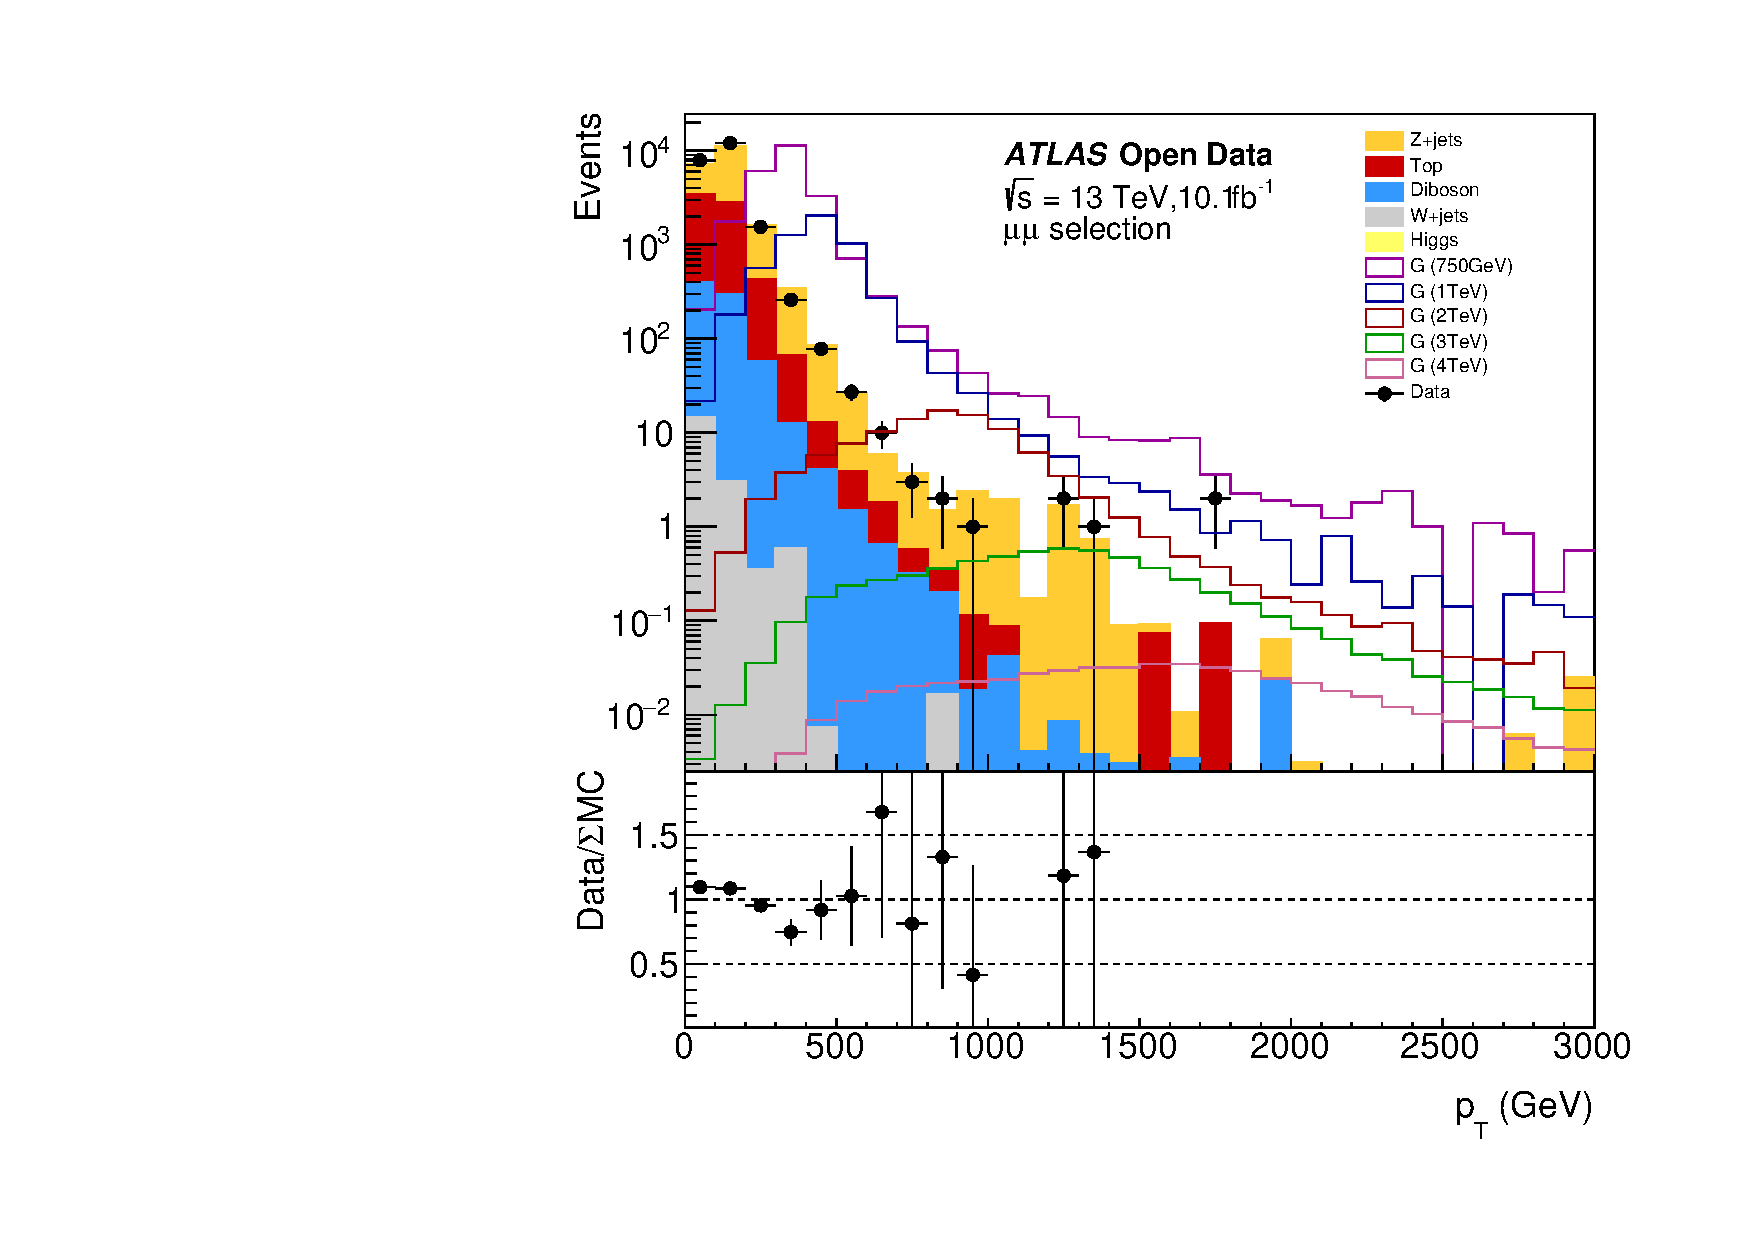
\includegraphics[width=1.1\textwidth]{../../Project3_test/Plots/all/uu_pt_all.pdf}
%       \caption[]%
%       {{\small Muon transverse momentum}}    
%       \label{fig:uu_pt_all}
    \end{subfigure}
    \hfill
    \begin{subfigure}[b]{0.475\textwidth}  
        \centering 
        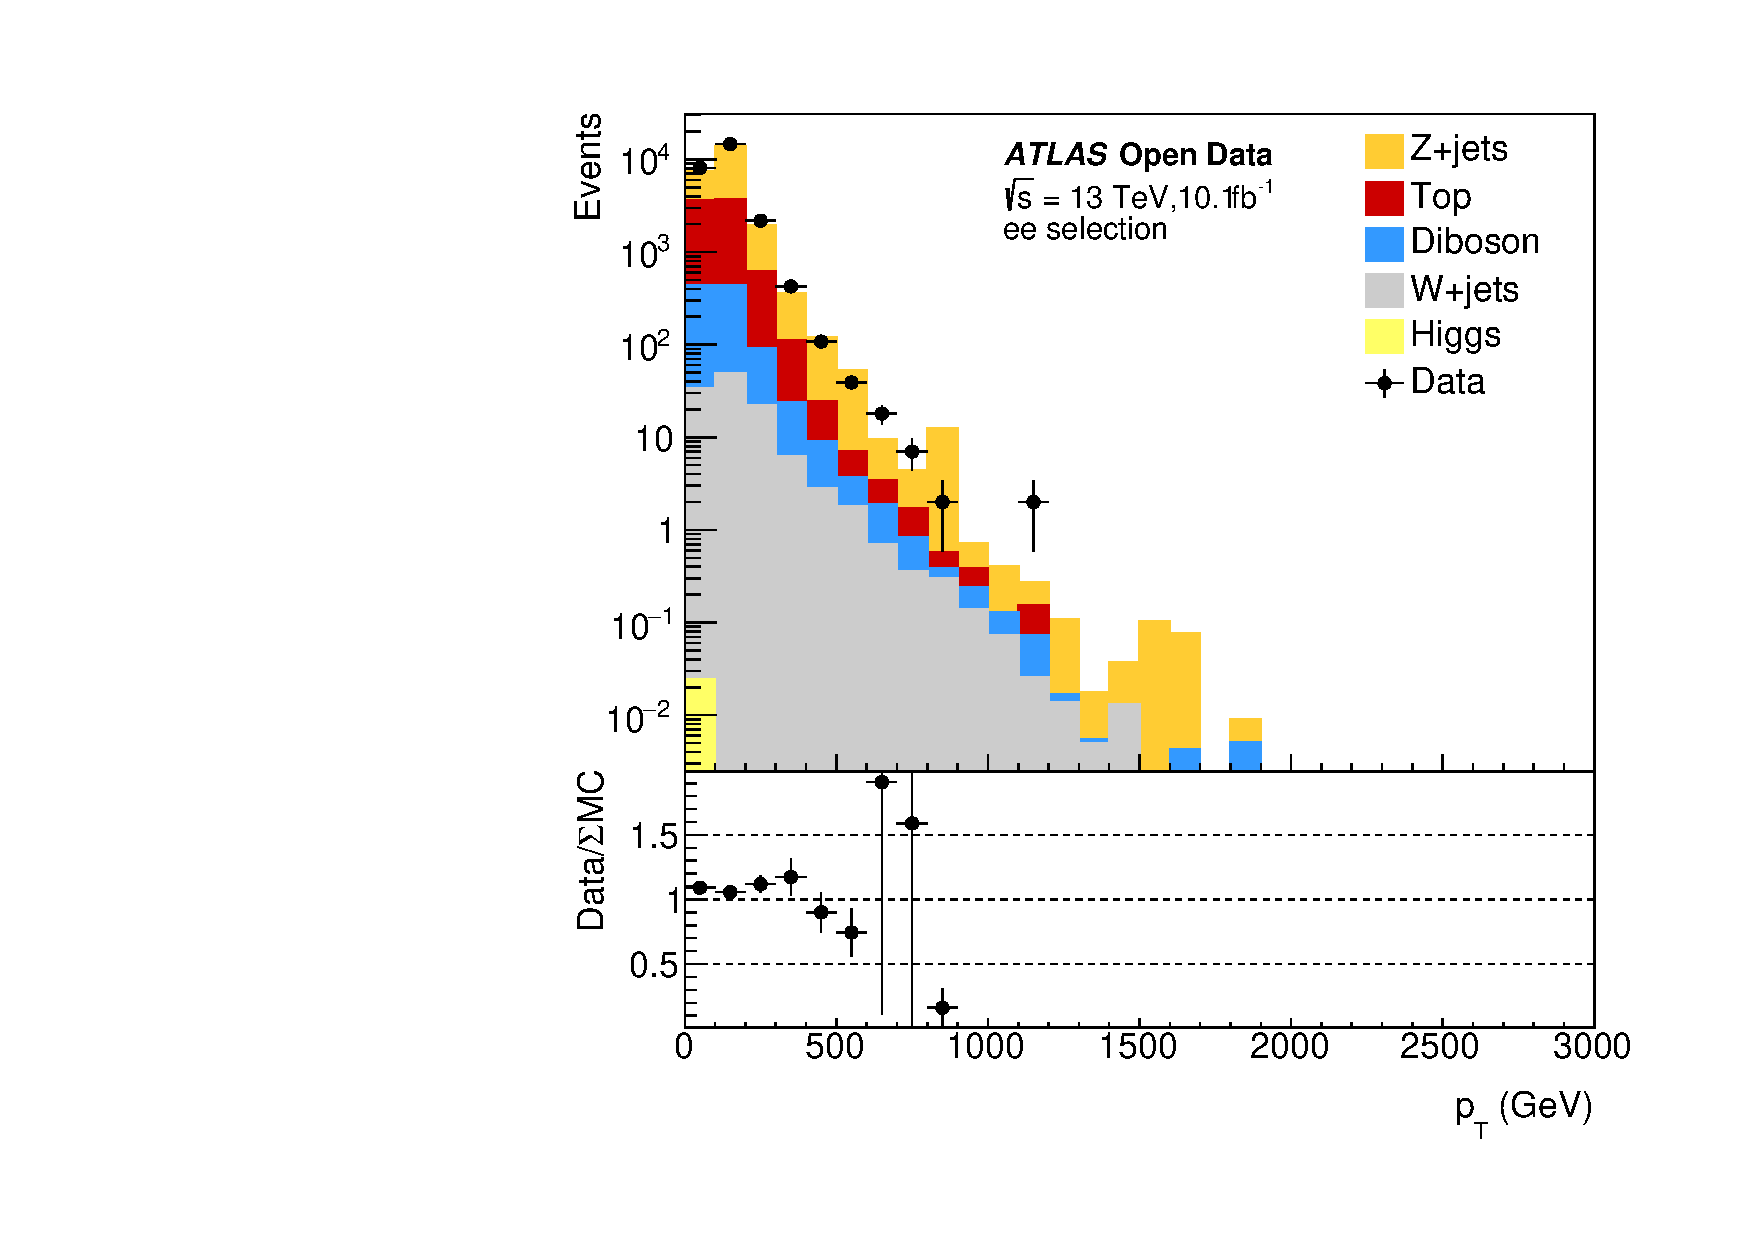
\includegraphics[width=1.1\textwidth]{../../Project3_test/Plots/all/ee_pt_all.pdf}
%        \caption[]%
%        {{\small Electron transverse momentum}}    
%        \label{fig:ee_pt_all}
    \end{subfigure}
%    \vskip\baselineskip
	~
    \begin{subfigure}[b]{0.475\textwidth}   
        \centering 
        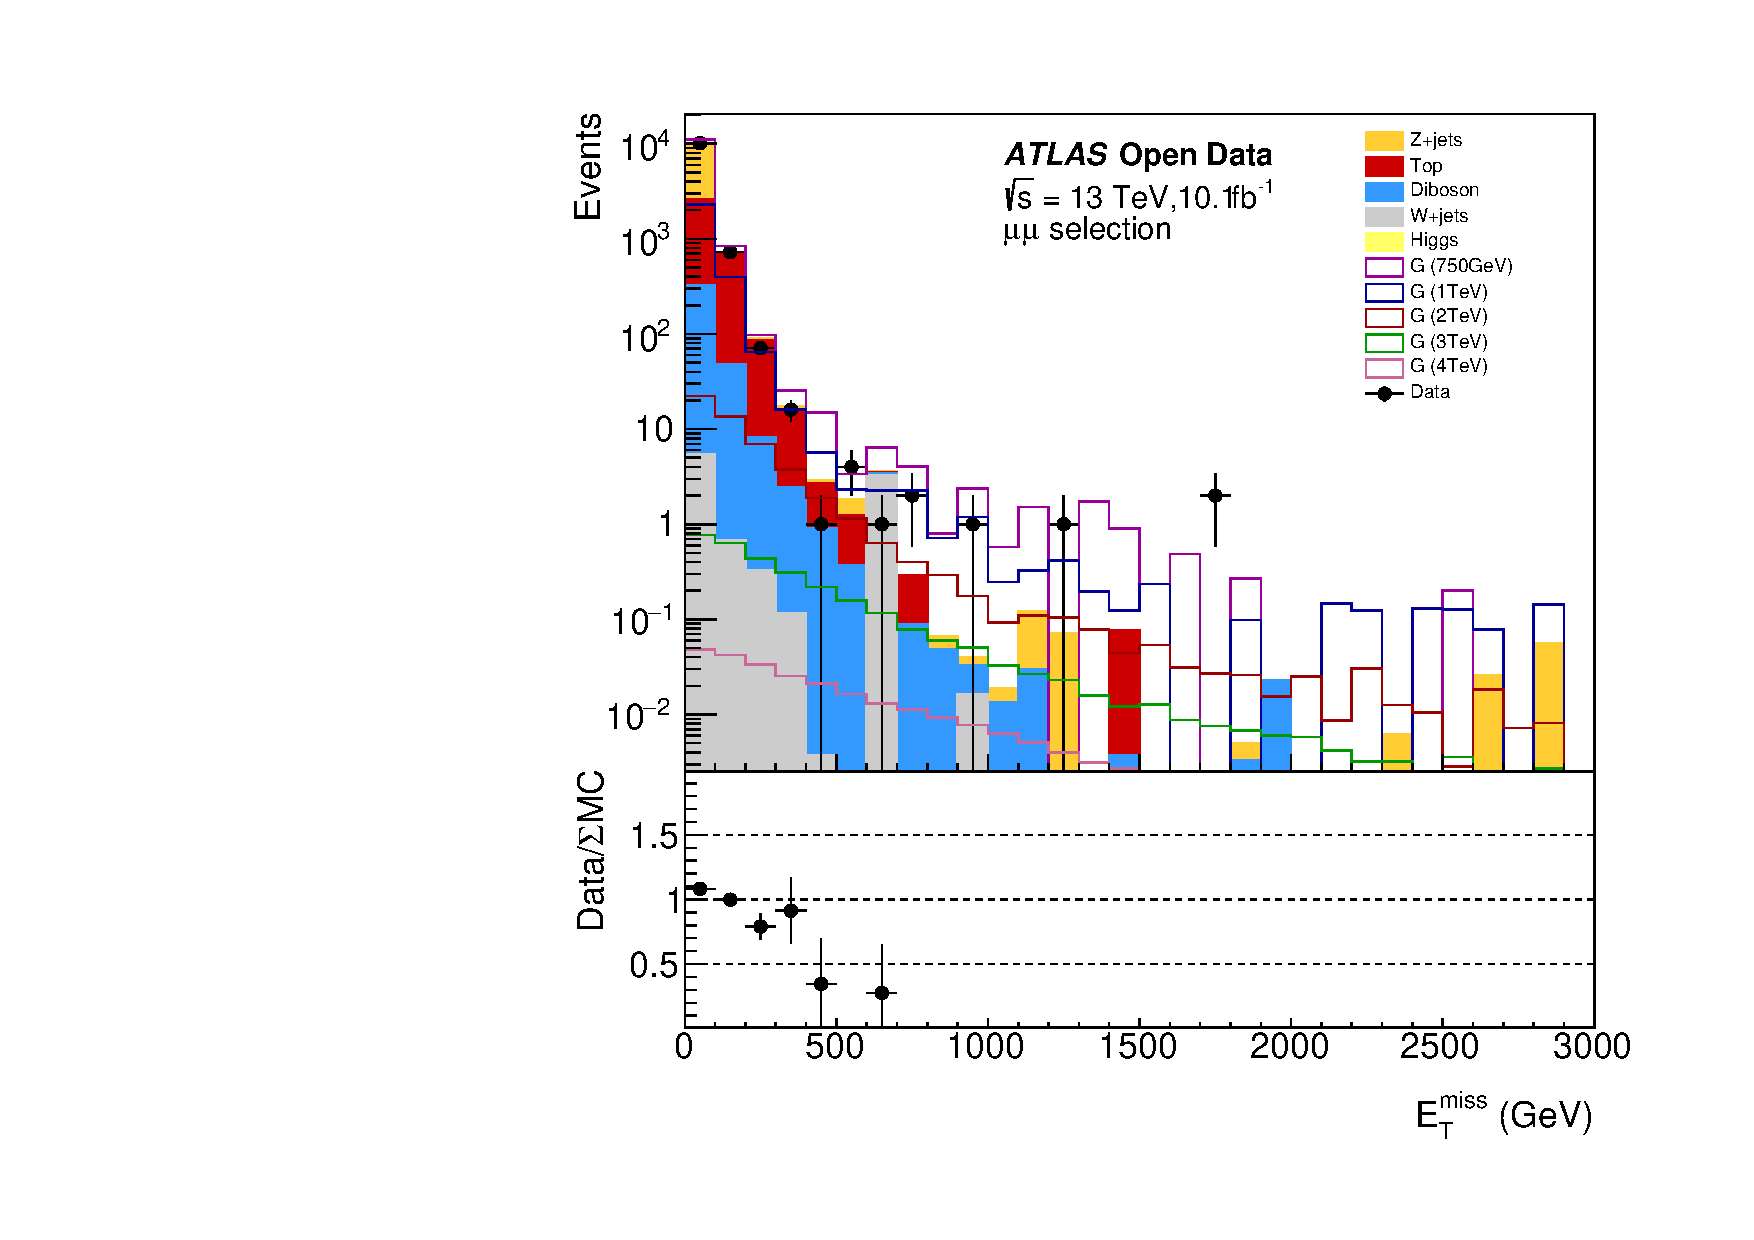
\includegraphics[width=1.1\textwidth]{../../Project3_test/Plots/all/uu_met_all.pdf}
%        \caption[]%
%        {{\small Network 3}}    
%        \label{fig:mean and std of net34}
    \end{subfigure}
    \quad
    \begin{subfigure}[b]{0.475\textwidth}   
        \centering 
        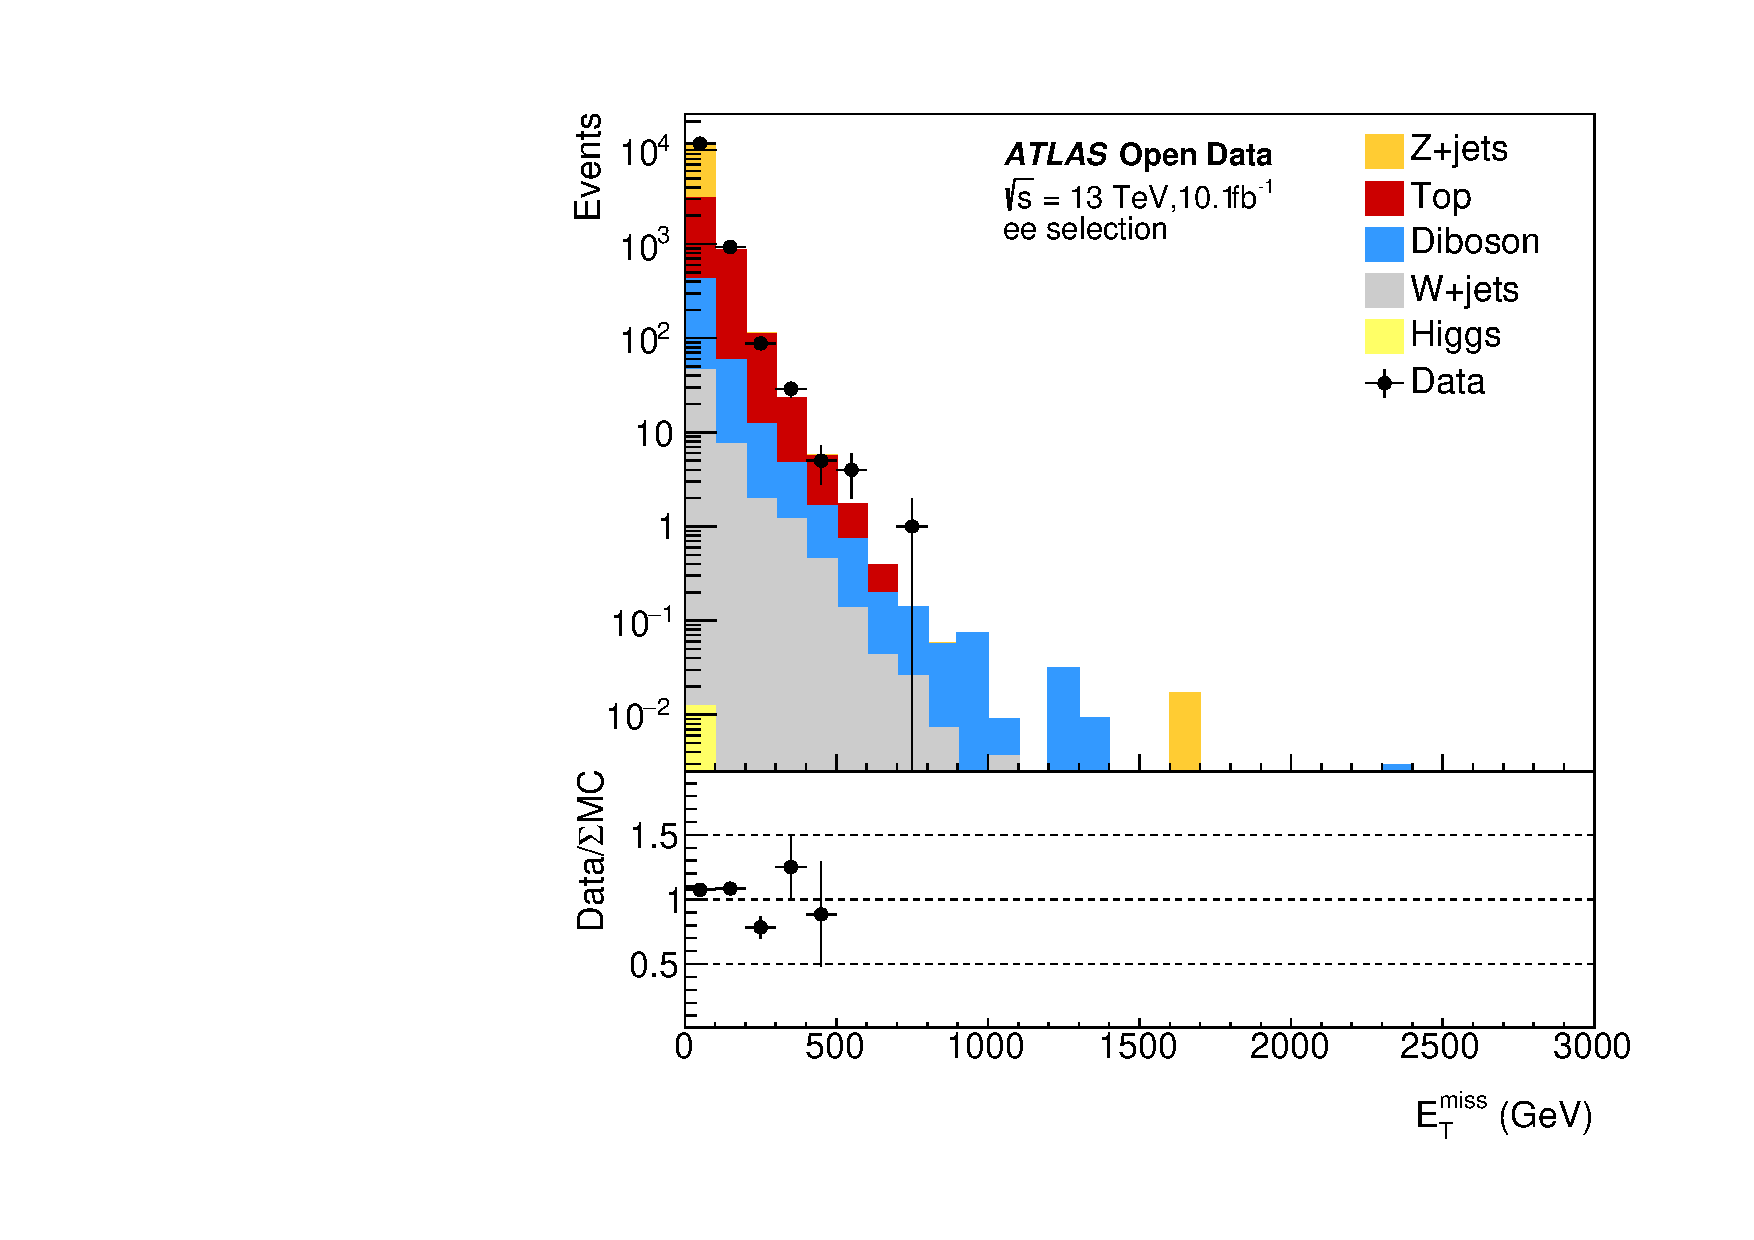
\includegraphics[width=1.1\textwidth]{../../Project3_test/Plots/all/ee_met_all.pdf}
%        \caption[]%
%        {{\small Network 4}}    
%        \label{fig:mean and std of net44}
    \end{subfigure}
%    \vskip\baselineskip
	~
    \begin{subfigure}[b]{0.475\textwidth}   
        \centering 
        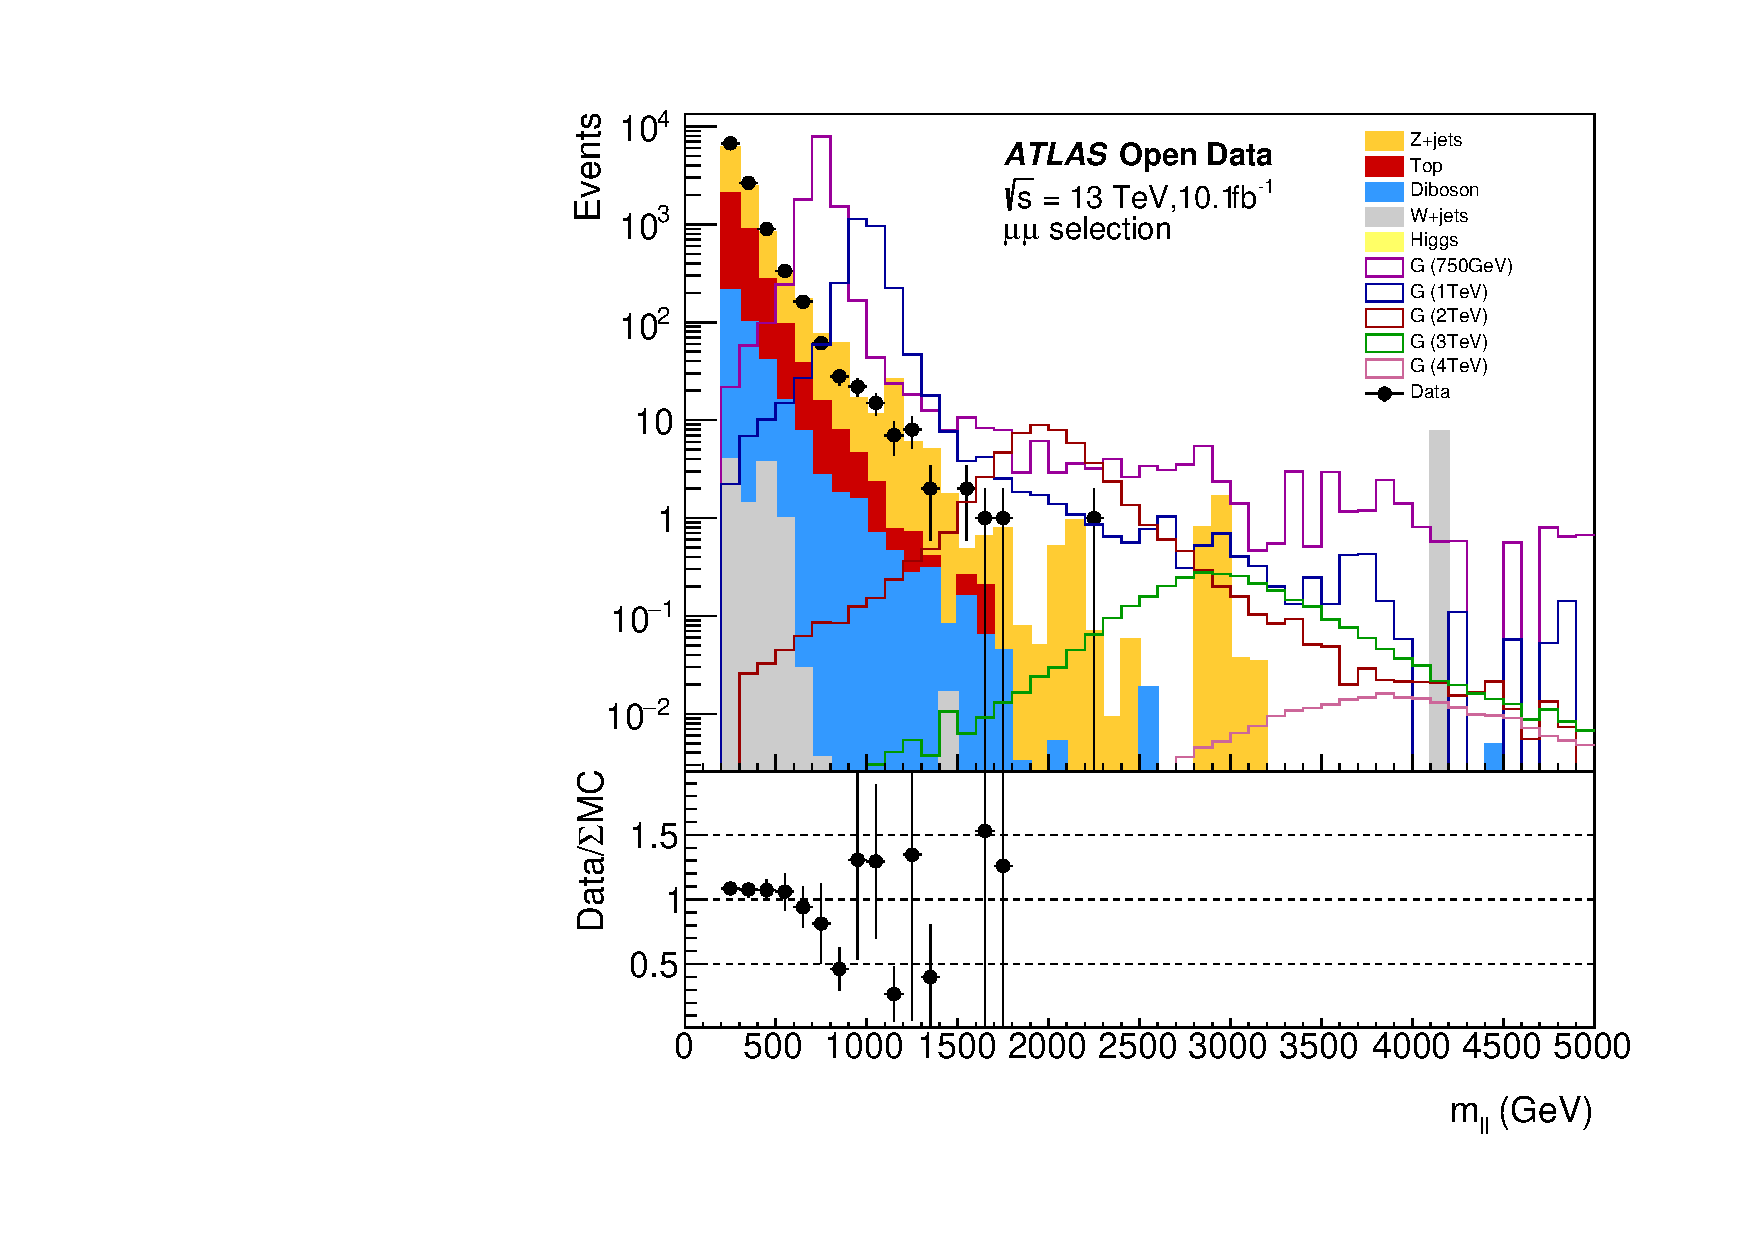
\includegraphics[width=1.1\textwidth]{../../Project3_test/Plots/all/uu_mll_all.pdf}
%        \caption[]%
%        {{\small Network 3}}    
%        \label{fig:mean and std of net34}
    \end{subfigure}
    \quad
    \begin{subfigure}[b]{0.475\textwidth}
        \centering 
        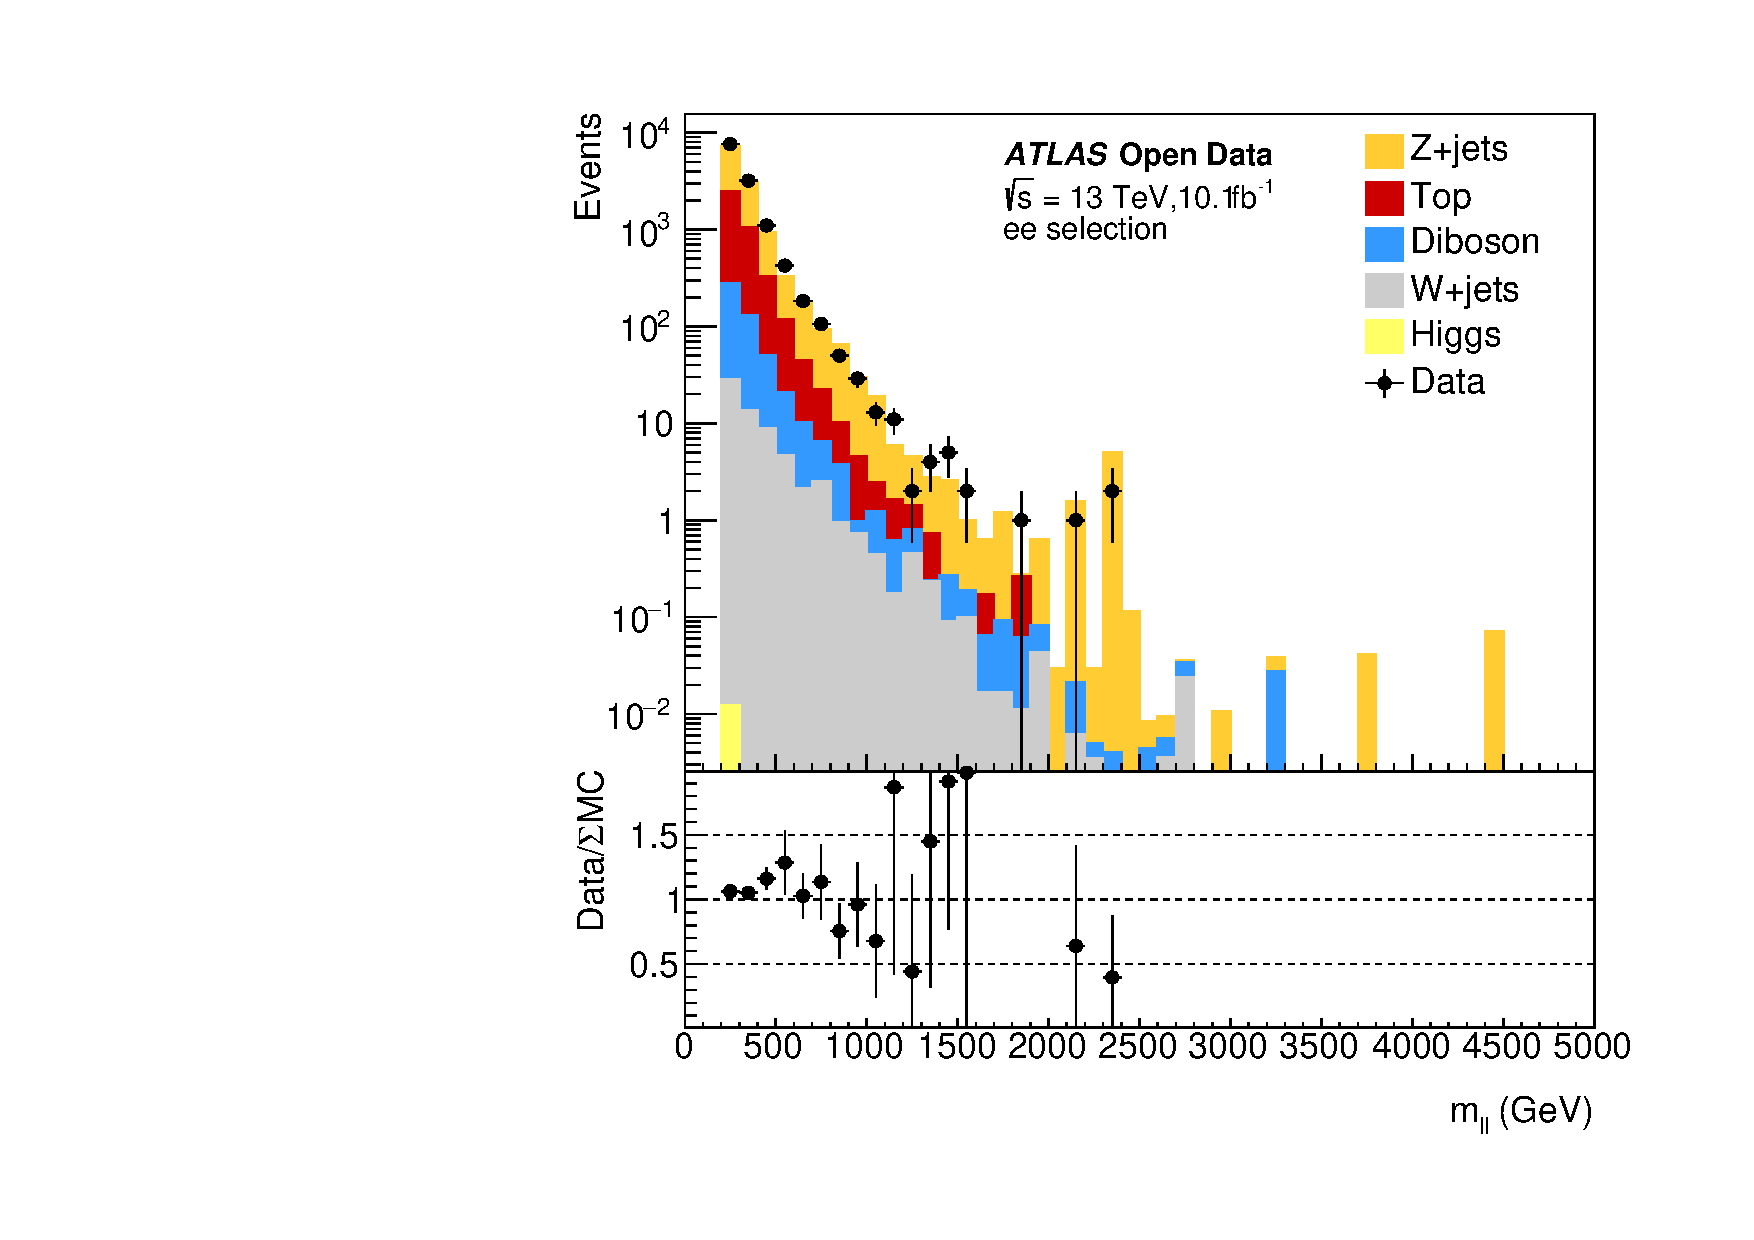
\includegraphics[width=1.1\textwidth]{../../Project3_test/Plots/all/ee_mll_all.pdf}
%        \caption[]%
%        {{\small Network 4}}    
%        \label{fig:mean and std of net44}
    \end{subfigure}
    \caption[ Parameters transverse momentum), missing transverse energy, and invariant mass ]
    {\small Parameters $p_T$, $E_T^{miss}$ and $m_{ll}$ for the electron ($e$) and muon ($\mu$) channel. } 
    \label{fig:lepton_parameters}
\end{figure*}
\restoregeometry 

\section{Discussion}
\section{Results}

\printbibliography

\end{document}

